% !TeX program = xelatex
\documentclass{article}
\usepackage{kotex}
\usepackage[a4paper, left=3cm, right=3cm, top=2.5cm, bottom=2.5cm]{geometry}
\usepackage{amsmath, amssymb}
\usepackage{tcolorbox}
\usepackage{caption}
\usepackage{setspace}
\usepackage{xcolor}
\usepackage{titlesec}
\usepackage{tikz}
\usetikzlibrary{arrows.meta}

\setstretch{1.3}
\renewcommand{\figurename}{그림}
\titleformat{name=\section,numberless}
  {\normalfont\large\bfseries\color{blue}}{}
  {0pt}{}

\title{1.5 평행 이동}
\date{}
\author{}

\begin{document}
\maketitle

\section*{1.5 평행 이동}

\begin{tcolorbox}[
  colback=teal!4, colframe=teal!65!black,
  title=정의 \& 핵심 규칙,
  fonttitle=\bfseries, boxrule=0.5mm, arc=3mm]

\textbf{\textcolor{teal!65!black}{정의 (평행 이동).}}\quad
$\mathbb{E}^n$에서 벡터 $\vec{v} \in \mathbb{R}^n$에 대응된 \textbf{평행 이동(translation)} $T$는
물체를 회전·향 변환 없이 곧은 직선을 따라 옮긴다.
\[
  T(P) \;=\; P + \vec{v}
\]
이 때 $\vec{v}$를 $T$의 \textbf{번위(변위) 벡터}라 부른다.

\noindent\textcolor{teal!50!black}{\rule{\linewidth}{0.4pt}}

\textbf{\textcolor{teal!65!black}{좌표 공식.}}\quad
$\vec{v} = (v_1, \ldots, v_n)$이면
\[
  T(x_1, \ldots, x_n) \;=\; (x_1 + v_1,\; \ldots,\; x_n + v_n)
\]

\noindent\textcolor{teal!50!black}{\rule{\linewidth}{0.4pt}}

\textbf{\textcolor{teal!65!black}{핵심 규칙 (합성과 역함수).}}
\begin{itemize}\setlength\itemsep{2pt}
  \item \textbf{합성}: $T_{\vec{v}} \circ T_{\vec{w}} = T_{\vec{v}+\vec{w}}$
        \hfill (평행 이동의 합성은 벡터의 합에 대응)
  \item \textbf{역함수}: $T_{\vec{v}}^{-1} = T_{-\vec{v}}$
        \hfill (역방향으로 같은 거리만큼 이동)
\end{itemize}

\end{tcolorbox}

\begin{figure}[h]
\centering
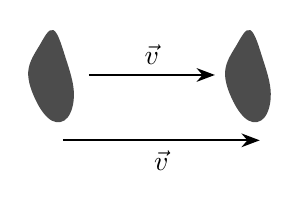
\begin{tikzpicture}[>=Stealth, scale=1.0]
  % Original shape (simple blob at left)
  \draw[fill=black!70, draw=none]
    plot[smooth cycle, tension=0.65] coordinates {
      (0.00,1.15)(-0.18,0.95)(-0.32,0.62)(-0.22,0.25)
      (-0.02,0.00)(0.18,0.04)(0.26,0.35)(0.16,0.78)
    };

  % Translation arrow v
  \draw[->, thick] (0.45,0.58) -- (2.05,0.58) node[midway,above]{$\vec{v}$};

  % Translated shape (same blob shifted right by 2.5)
  \begin{scope}[xshift=2.5cm]
    \draw[fill=black!70, draw=none]
      plot[smooth cycle, tension=0.65] coordinates {
        (0.00,1.15)(-0.18,0.95)(-0.32,0.62)(-0.22,0.25)
        (-0.02,0.00)(0.18,0.04)(0.26,0.35)(0.16,0.78)
      };
  \end{scope}

  % Second translation arrow v (bottom)
  \draw[->, thick] (0.12,-0.25) -- (2.62,-0.25) node[midway,below]{$\vec{v}$};
\end{tikzpicture}
\caption{벡터 $\vec{v}$에 의한 평행 이동}
\label{fig:1.10}
\end{figure}

\begin{tcolorbox}[
  colback=red!4, colframe=red!60!black,
  title=정리 1.5.1\quad 두 평행 직선의 반사 합성,
  fonttitle=\bfseries, boxrule=0.5mm, arc=3mm]

$\mathbb{E}^2$에서 평행한 두 직선 $L_1$, $L_2$에 대해
$\vec{v}$를 $L_1$ 위의 한 점을 시점, $L_2$ 위의 한 점을 종점으로 하되
두 직선과 각각 수직으로 만나는 벡터라 하자.
$f_1$을 $L_1$에 대한 반사, $f_2$를 $L_2$에 대한 반사라 하면,
\[
  f_2 \circ f_1 \;=\; T_{2\vec{v}} \qquad \text{(벡터 $2\vec{v}$에 의한 평행 이동)}
\]

\end{tcolorbox}

\textbf{증명.}\quad $P$를 임의의 점이라 하자.
$\vec{A}$와 $\vec{B}$를 두 직선에 수직인 벡터로,
$\vec{A}$는 $P$를 시점으로 $L_1$의 한 점을 종점으로 하고
$\vec{B}$는 $f_1(P)$를 시점으로 $L_2$의 한 점을 종점으로 한다고 하자.
그러면 다음을 얻는다.
\[
  P + \vec{A} \in L_1, \qquad
  P + 2\vec{A} = f_1(P), \qquad
  P + 2\vec{A} + \vec{B} \in L_2, \qquad
  P + 2\vec{A} + 2\vec{B} = f_2(f_1(P))
\]
$\vec{A}+\vec{B}$는 $L_1$의 점을 시점으로 $L_2$의 점을 종점으로 하는 벡터로 볼 수 있고,
세 벡터 $\vec{v}$, $\vec{A}$, $\vec{B}$는 모두 $L_1$과 $L_2$에 수직이므로
$\vec{v} = \vec{A}+\vec{B}$임을 알 수 있다.
따라서 임의의 점 $P$에 대해 $f_2(f_1(P)) = P + 2\vec{v}$가 성립한다.
\hfill $\square$

\smallskip
$\mathbb{E}^3$에서 평행한 평면에 대한 반사에 대해서도 비슷한 정리와 비슷한 증명이 성립한다.

\subsection*{연습문제 1.5}

\begin{enumerate}
  \item \textbf{(문제 1.5.2)}\quad 정리 1.5.1에서 $f_1 \circ f_2$를 기술하여라.

  \item \textbf{(문제 1.5.3)}\quad $\mathbb{E}^2$에서 직선 $L$과 $L$에 평행한 벡터 $\vec{v}$에 대해
    다음이 성립함을 보여라.
    \[
      T_{\vec{v}} \circ f_L = f_L \circ T_{\vec{v}}
      \qquad (f_L \text{은 직선 } L \text{에 대한 반사})
    \]
    위 문제에서의 변환 $T_{\vec{v}} \circ f_L$을 $L$과 $\vec{v}$에 의한 \textbf{미끄럼 반사}라 한다.
\end{enumerate}

\end{document}
